\documentclass[11pt]{article}

% ============================================================================
% PACKAGES
% ============================================================================
\usepackage[margin=1in]{geometry}
\usepackage{graphicx}
\usepackage{hyperref}
\usepackage{booktabs}
\usepackage{longtable}
\usepackage{enumitem}
\usepackage{xcolor}
\usepackage{fancyhdr}

\graphicspath{{../../screenshots/}{../../analysis/figures/}}

% ============================================================================
% DOCUMENT SETTINGS
% ============================================================================
\hypersetup{
    colorlinks=true,
    linkcolor=blue,
    urlcolor=blue,
    citecolor=blue
}

\pagestyle{fancy}
\fancyhf{}
\rhead{EECE 5155 -- Final Deliverable}
\lhead{Spring 2026}
\cfoot{\thepage}

% ============================================================================
% TITLE BLOCK
% ============================================================================
\title{%
    \textbf{EECE 5155: Wireless Sensor Networks and IoT Systems}\\[0.5em]
    \Large Final Deliverable -- Pipeline + ML/AI\\[1em]
    \large \textit{TrekTrak: Bike Path Pedestrian \& Cyclist Traffic Monitor}
}

\author{%
    \textbf{Student Name:} William Rice\\
    \textbf{NUID:} 002856676\\
    \textbf{GitHub Repo:} \url{https://github.com/ricewillwin/TrekTrak}\\
    \textbf{Date:} 2026-04-23\\
    \textbf{Version:} 1.0
}

\date{}

\begin{document}

\maketitle
\thispagestyle{fancy}

% %%%%%%%%%%%%%%%%%%%%%%%%%%%%%%%%%%%%%%%%%%%%%%%%%%%%%%%%%%%%%%%%%%%%%%%%%%%%
%
%   PART A: DATA PIPELINE (15 points)
%
% %%%%%%%%%%%%%%%%%%%%%%%%%%%%%%%%%%%%%%%%%%%%%%%%%%%%%%%%%%%%%%%%%%%%%%%%%%%%

\part*{Part A: Data Pipeline and Cloud Integration (15 points)}
\addcontentsline{toc}{part}{Part A: Data Pipeline}

% ============================================================================
% SECTION 1: SYSTEM ARCHITECTURE AND NODE-RED
% ============================================================================
\section{System Architecture and Node-RED Flow}
\label{sec:architecture}

\noindent\textbf{E1 Reference:} Commit hash \texttt{273a3c4} --- Changes since E1: Added Docker Compose pipeline stack (Mosquitto MQTT broker, InfluxDB~v2, Node-RED, Grafana, Traefik reverse proxy); Python simulation script (\texttt{simulation/simulation.py}) for generating and publishing synthetic 24-hour traffic data; updated Node-RED flow with InfluxDB out nodes for each sensor type.

\vspace{0.5em}

\noindent\textbf{Data Flow:}
\begin{enumerate}[noitemsep]
    \item \textbf{Simulation $\to$ MQTT:} \texttt{simulation/simulation.py} publishes JSON payloads to topic \texttt{trektrak/sensor/report} on the Mosquitto broker (port~1883). Each payload contains \texttt{seq}, \texttt{gps} (lat, lon), \texttt{ultrasonic} (detections, total\_presence\_sec), \texttt{pir} (triggers), and \texttt{uptime\_sec}. Reports represent 15-minute windows; \texttt{--fast} mode publishes all 96 daily windows at 1-second real-time intervals.
    \item \textbf{MQTT $\to$ Node-RED:} Node-RED subscribes to \texttt{trektrak/sensor/report} on the Mosquitto container (internal hostname \texttt{mosquitto}, port~1883). A JSON node converts the raw string payload into a JavaScript object.
    \item \textbf{Node-RED $\to$ InfluxDB:} Three function nodes extract sensor sub-objects and route them to separate InfluxDB~v2 out nodes: \textit{Ultrasonic Sensor} (fields \texttt{detections}, \texttt{total\_presence\_sec} $\to$ measurement \texttt{ultrasonic}), \textit{PIR Sensor} (field \texttt{triggers} $\to$ measurement \texttt{pir}), and \textit{GPS Sensor} (fields \texttt{lat}, \texttt{lon} $\to$ measurement \texttt{gps}). All write to bucket \texttt{sensor}, organisation \texttt{trektrak}.
    \item \textbf{Node-RED $\to$ CSV:} CSV export is not implemented as a Node-RED node. Data can be exported from the simulation directly using \texttt{simulation.py --csv data/sim.csv}, which writes all generated reports to a local file for offline analysis.
    \item \textbf{InfluxDB $\to$ Grafana:} A Grafana Flux datasource connects to InfluxDB. The dashboard (\textit{Busyness}) contains three panels: a heatmap of detection counts, a time-series of detections and presence duration, and a time-series comparing PIR triggers to ultrasonic detections, all with auto-refresh enabled.
\end{enumerate}

\vspace{0.5em}

\noindent\textbf{Node-RED Flow Description:}\\{}
The exported flow (\texttt{analysis/nodered.json}) subscribes to \texttt{trektrak/sensor/report} via an MQTT~In node connected to the Mosquitto service. A JSON parse node fans the parsed payload out to three function nodes. Each function node extracts one sensor sub-object (\texttt{msg.payload.ultrasonic}, \texttt{msg.payload.pir}, \texttt{msg.payload.gps}) and passes it to both a debug node and an InfluxDB~v2 out node configured with the correct measurement name. The completed flow is shown in Figure~\ref{fig:nodered}.

\begin{figure}[htbp]
    \centering
    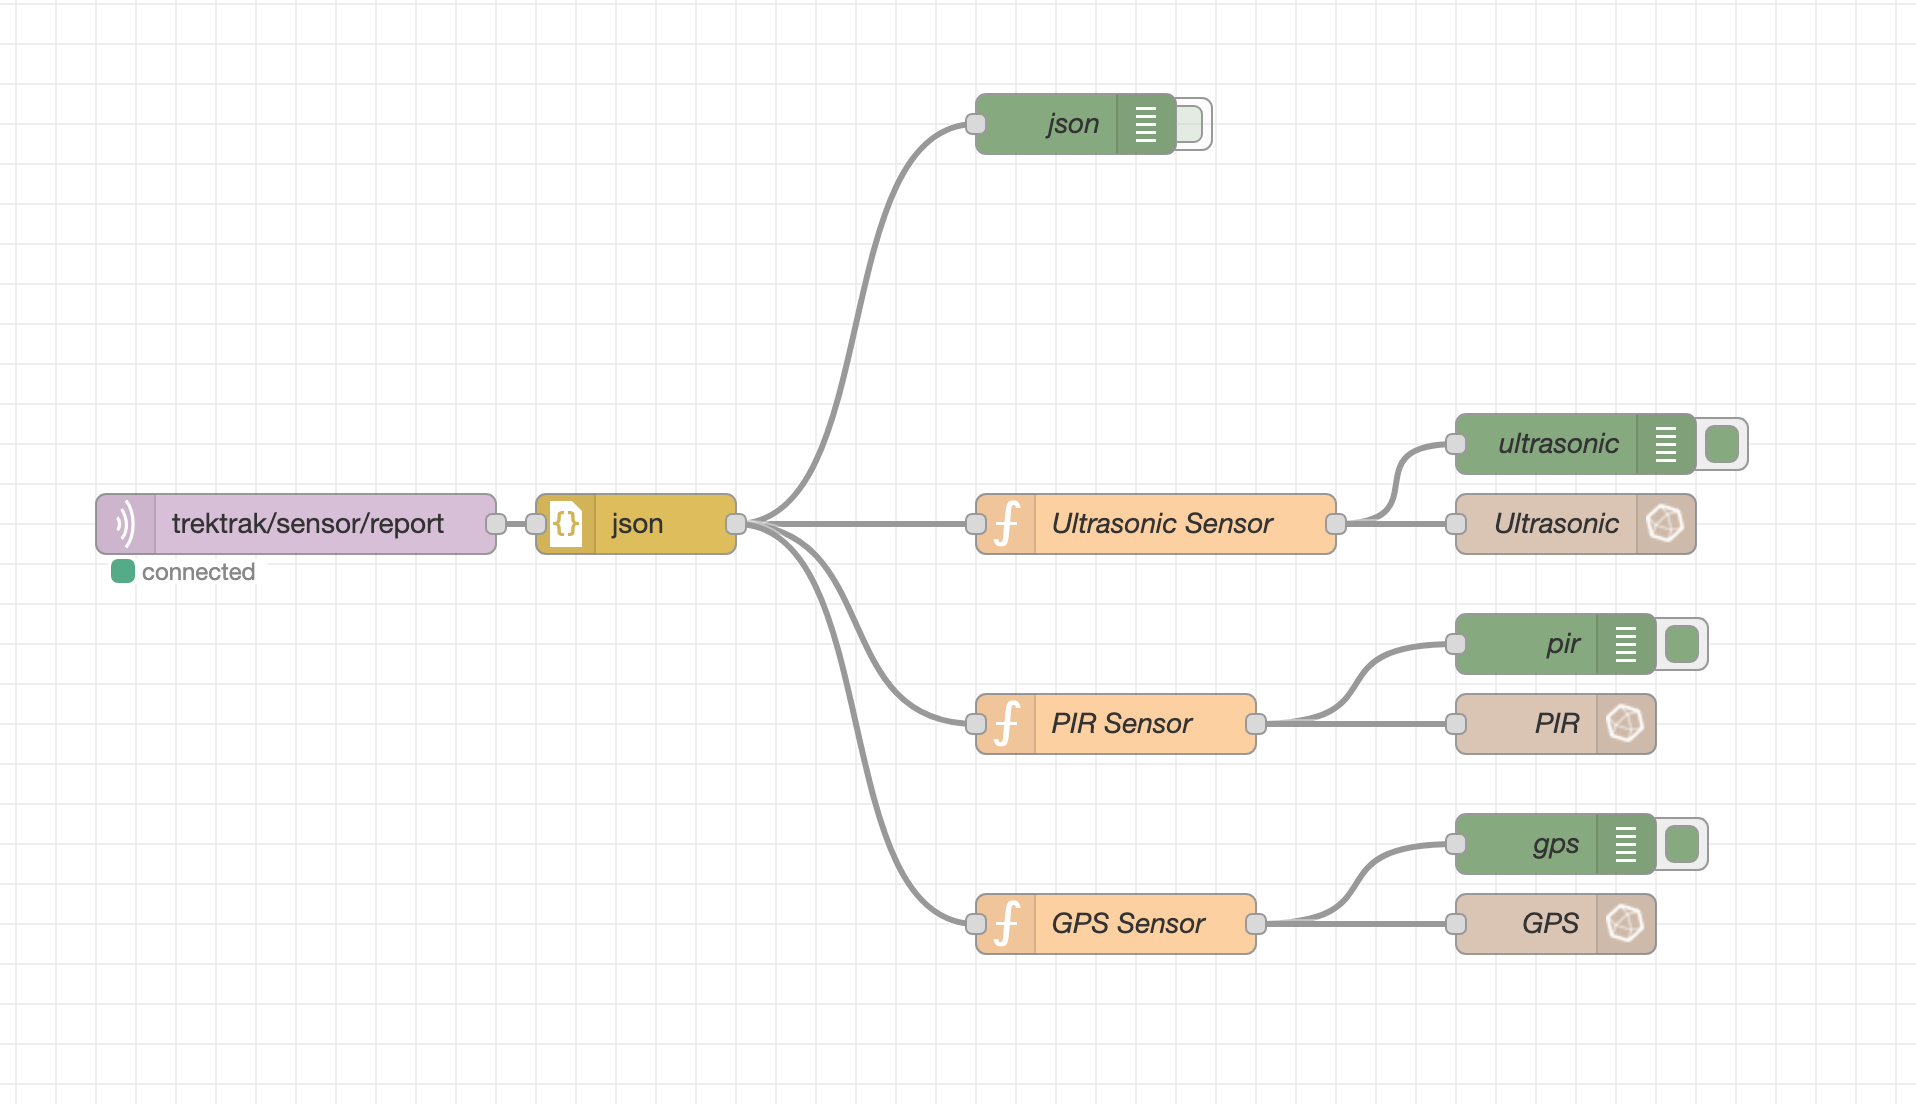
\includegraphics[width=0.92\textwidth]{final_node-red_flow.png}
    \caption{Final Node-RED flow: MQTT~In $\to$ JSON parse $\to$ Ultrasonic / PIR / GPS function nodes $\to$ InfluxDB out nodes.}
    \label{fig:nodered}
\end{figure}

Initial deployment hit an \texttt{HttpError: unauthorized access} when the InfluxDB out nodes first attempted to write (Figure~\ref{fig:autherror}). The root causes were two-fold: the default InfluxDB token had insufficient permissions, and the node was pointed at \texttt{localhost} rather than the InfluxDB container. Both were fixed by generating a custom all-access API token in the InfluxDB UI and updating the node's server address to the host's LAN IP. After that, data appeared in InfluxDB immediately.

\begin{figure}[htbp]
    \centering
    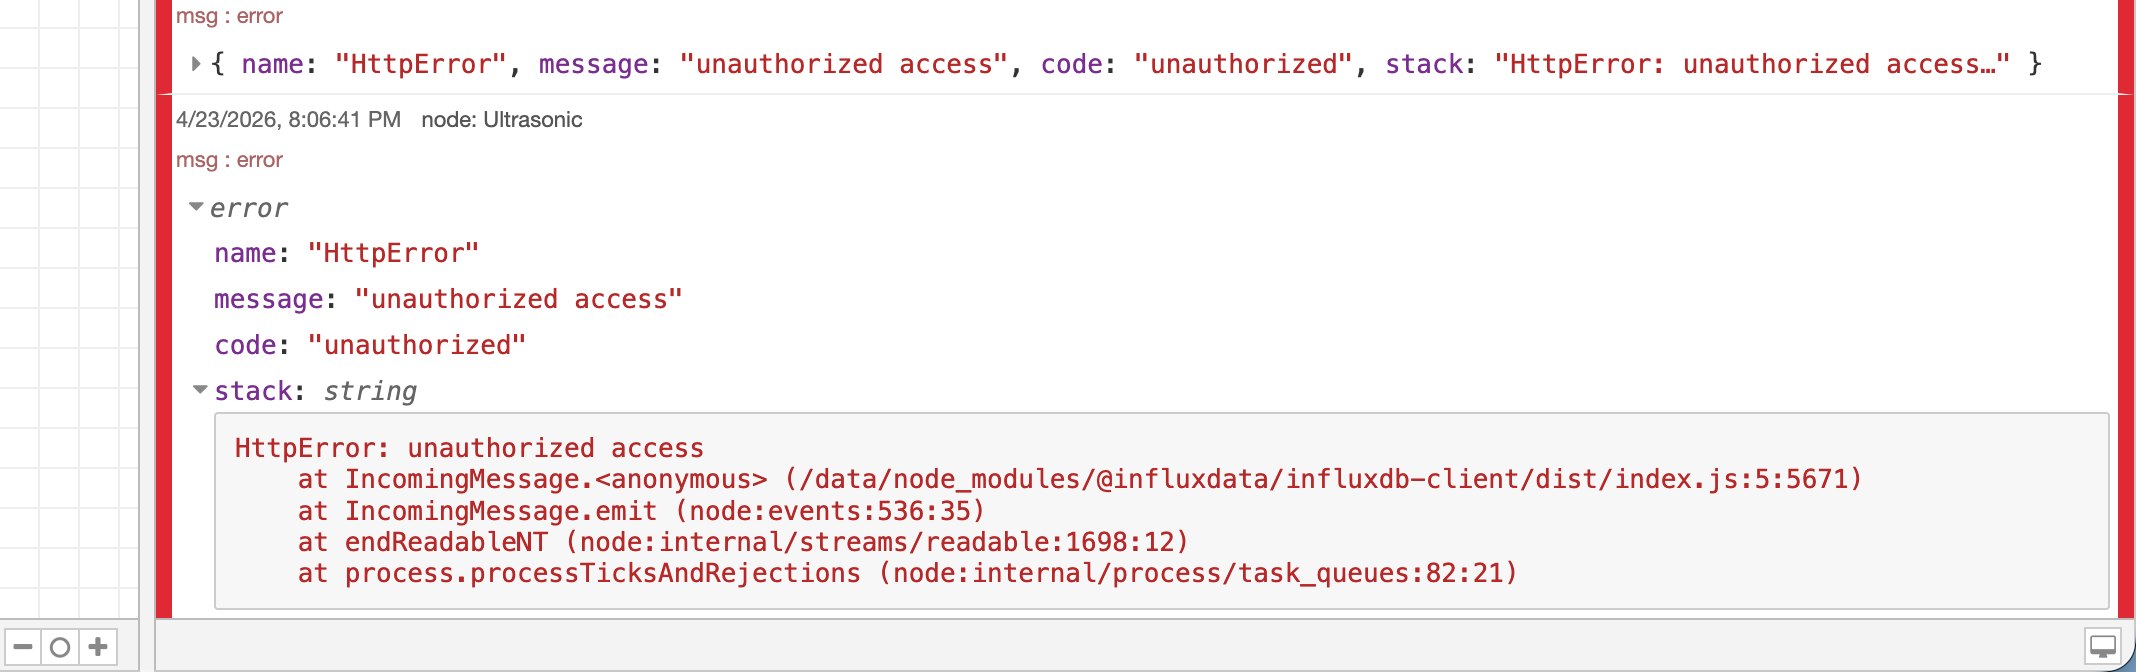
\includegraphics[width=0.85\textwidth]{error_attempting_to_connect_nodered-influx.png}
    \caption{Node-RED debug panel showing \texttt{HttpError: unauthorized access} on initial InfluxDB connection attempt.}
    \label{fig:autherror}
\end{figure}

\vspace{0.5em}

\noindent\textbf{Flow Export:} \texttt{analysis/nodered.json}

% ============================================================================
% SECTION 2: INFLUXDB AND GRAFANA
% ============================================================================
\section{InfluxDB Configuration and Grafana Dashboard}
\label{sec:storage}

InfluxDB~v2 runs as a Docker service initialised with organisation \texttt{trektrak} and bucket \texttt{sensor}. Three measurements are written by Node-RED: \texttt{ultrasonic} (detection count and presence duration), \texttt{pir} (trigger count), and \texttt{gps} (coordinates). No tags are used; with a single simulated sensor node the measurement name alone distinguishes the data streams. Data appears queryable in the InfluxDB Data Explorer within seconds of a simulation run (Figure~\ref{fig:influxdb}).

Connecting Grafana to InfluxDB was straightforward after the auth issues encountered in Node-RED had already been resolved --- the same API token and LAN IP were reused for the Flux datasource. The resulting dashboard (Figure~\ref{fig:grafana}) provides a clear view of simulated trail activity.

\vspace{0.5em}

% TABLE: InfluxDB Schema
\begin{table}[htbp]
\centering
\caption{InfluxDB Schema}
\label{tab:influx}
\begin{tabular}{@{}p{3cm}p{4cm}p{5cm}@{}}
\toprule
\textbf{Component} & \textbf{Name} & \textbf{Description} \\
\midrule
Organisation & trektrak & Project organisation \\
\addlinespace
Bucket & sensor & All sensor data for this project \\
\addlinespace
Measurement & ultrasonic & Per-window ultrasonic detection readings \\
\addlinespace
Measurement & pir & Per-window PIR trigger readings \\
\addlinespace
Field: detections & detections & Ultrasonic object detection count per 15-min window (count) \\
\addlinespace
Field: total\_presence\_sec & total\_presence\_sec & Accumulated detected presence per window (seconds) \\
\addlinespace
Field: triggers & triggers & PIR motion trigger count per 15-min window (count) \\
\bottomrule
\end{tabular}
\end{table}

\noindent\textbf{Sample Flux Query:}
\begin{verbatim}
from(bucket: "sensor")
  |> range(start: -1h)
  |> filter(fn: (r) => r._measurement == "ultrasonic")
  |> filter(fn: (r) => r._field == "detections")
  |> aggregateWindow(every: 15m, fn: mean, createEmpty: false)
\end{verbatim}

\vspace{0.5em}

% TABLE: Grafana Panels
\begin{table}[htbp]
\centering
\caption{Grafana Dashboard Panels}
\label{tab:panels}
\begin{tabular}{@{}p{0.5cm}p{3.5cm}p{4.5cm}p{3cm}@{}}
\toprule
\textbf{\#} & \textbf{Title} & \textbf{Data Shown} & \textbf{Visualization} \\
\midrule
1 & Detections (Busyness) & Ultrasonic detection count per window mapped to colour intensity & Heatmap \\
\addlinespace
2 & Detections and Length of Detections & \texttt{detections} and \texttt{total\_presence\_sec} over time & Time series \\
\addlinespace
3 & PIR Detections and Ultrasonic Detections & \texttt{pir.triggers} and \texttt{ultrasonic.detections} overlaid & Time series \\
\bottomrule
\end{tabular}
\end{table}

\begin{figure}[htbp]
    \centering
    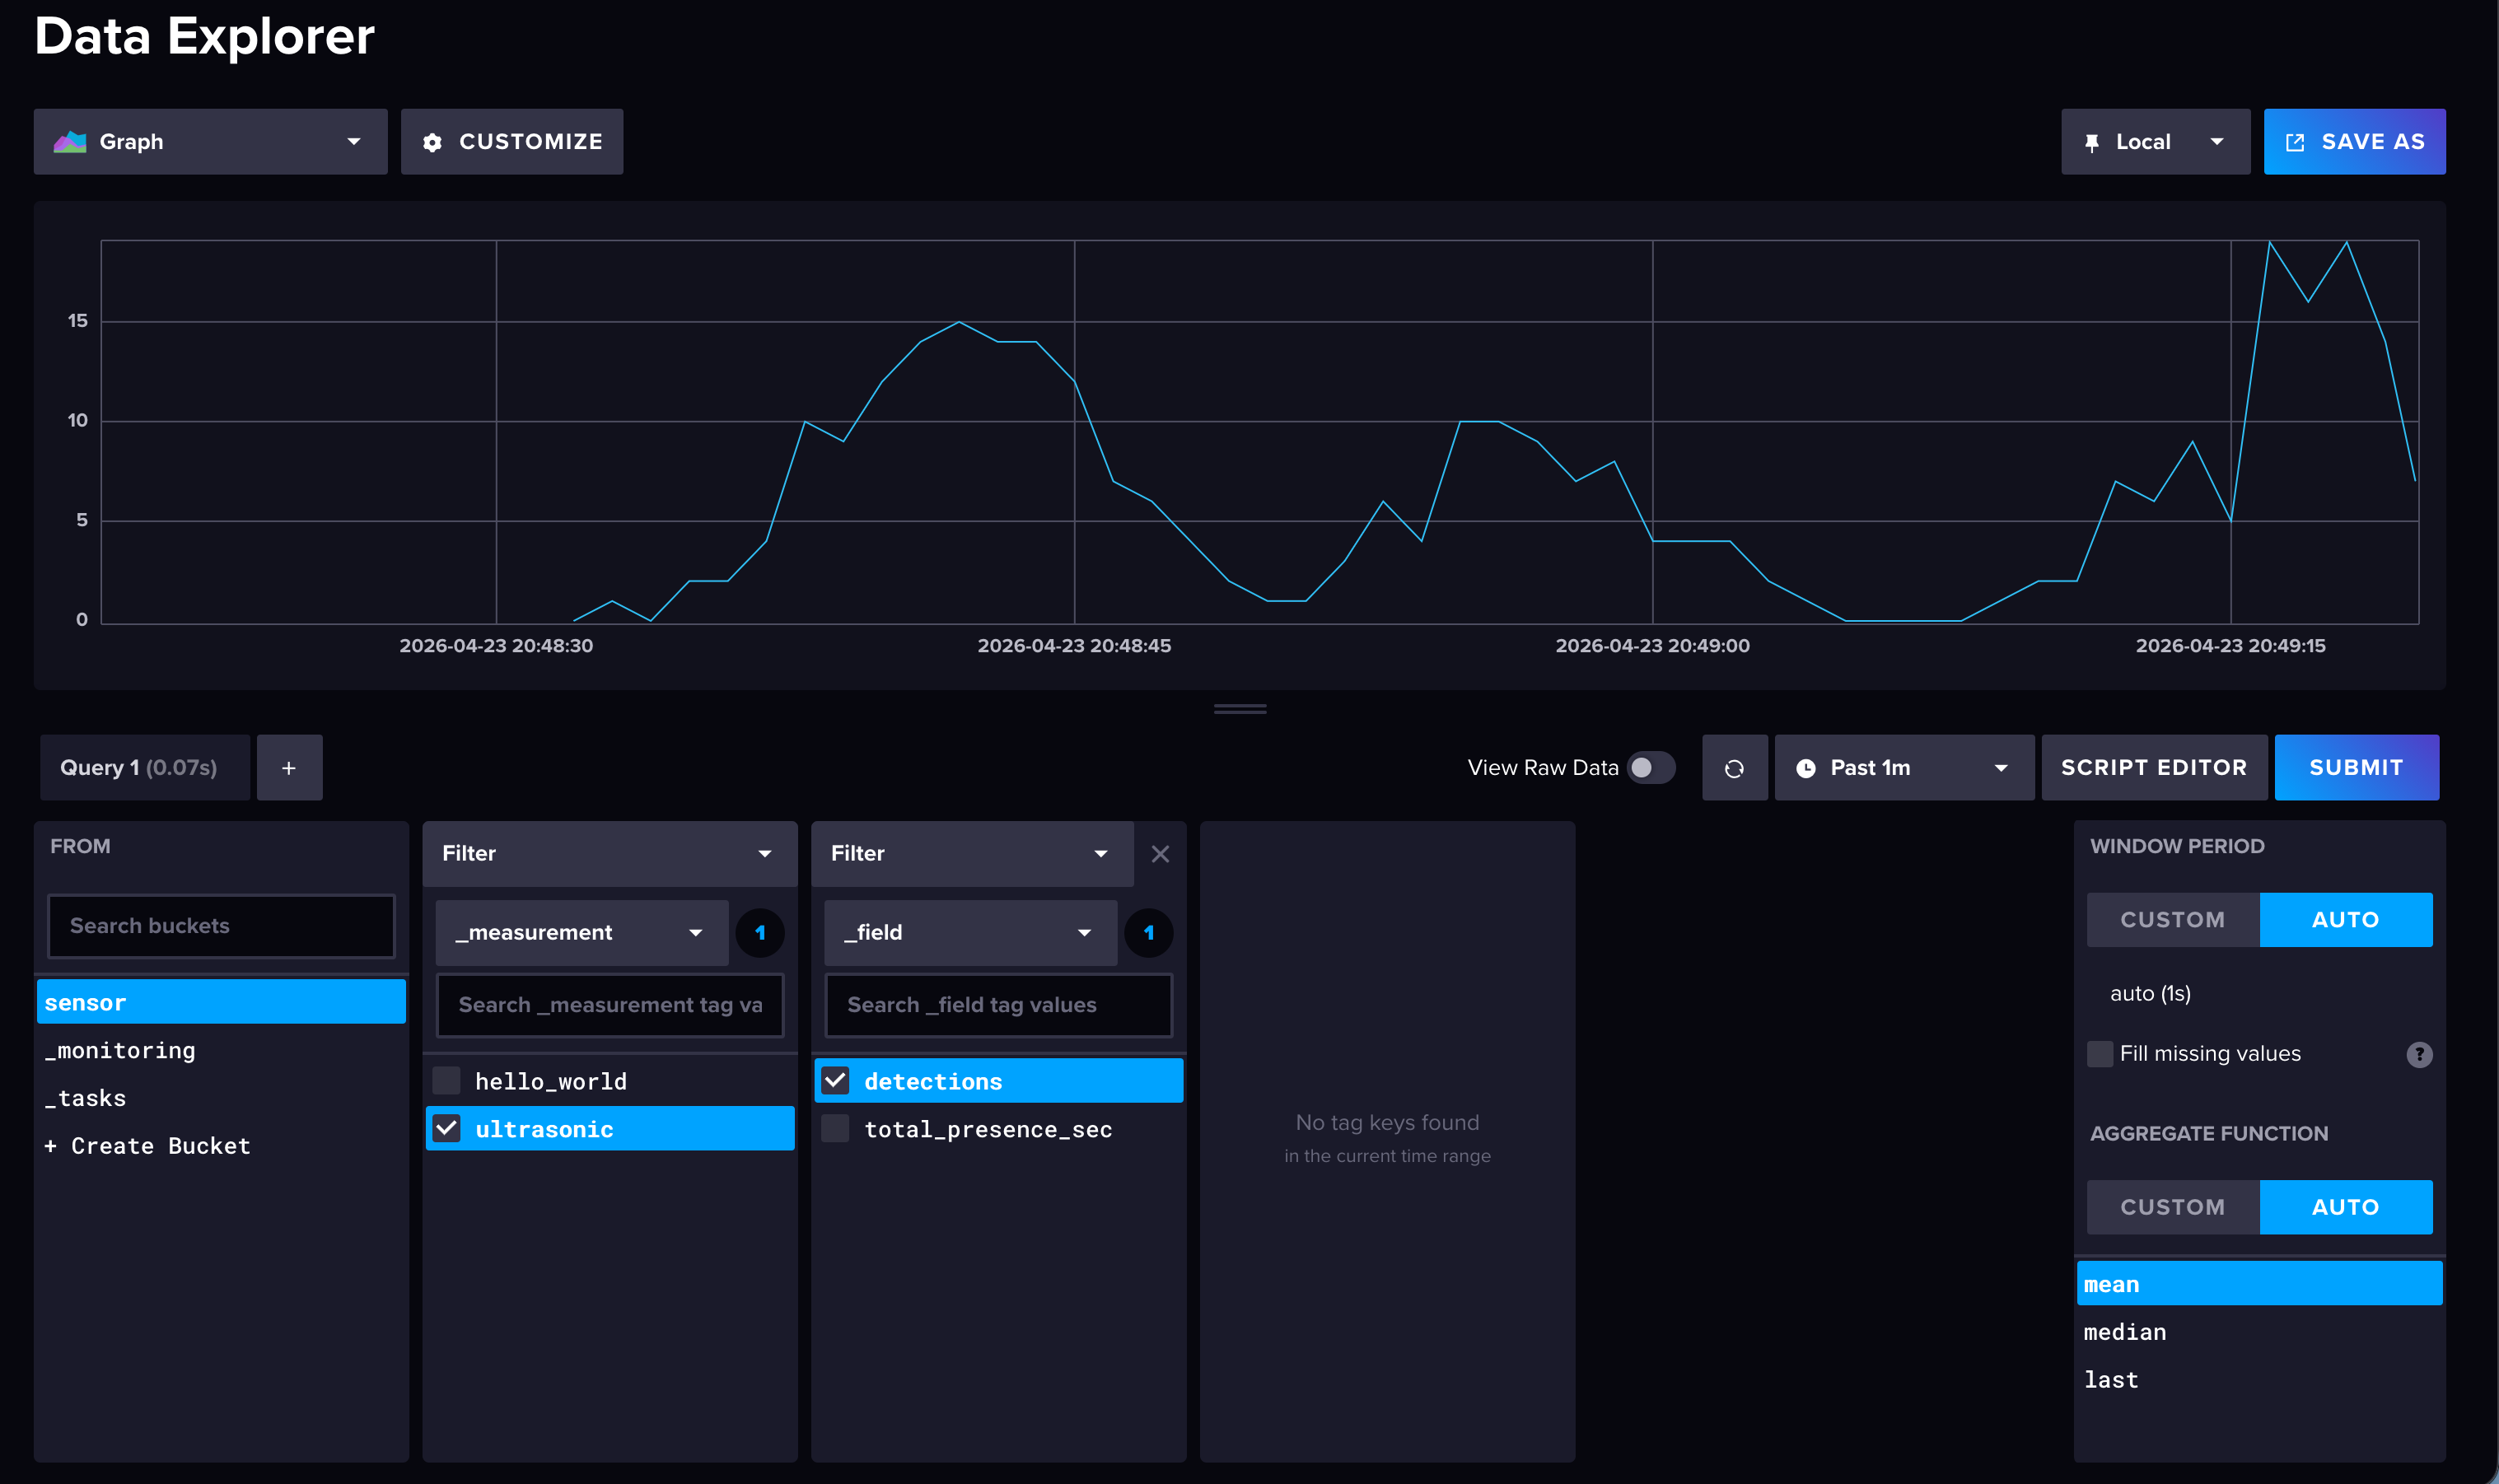
\includegraphics[width=0.92\textwidth]{data_in_influxdb.png}
    \caption{InfluxDB Data Explorer showing the \texttt{ultrasonic} measurement with \texttt{detections} field in the \texttt{sensor} bucket.}
    \label{fig:influxdb}
\end{figure}

\begin{figure}[htbp]
    \centering
    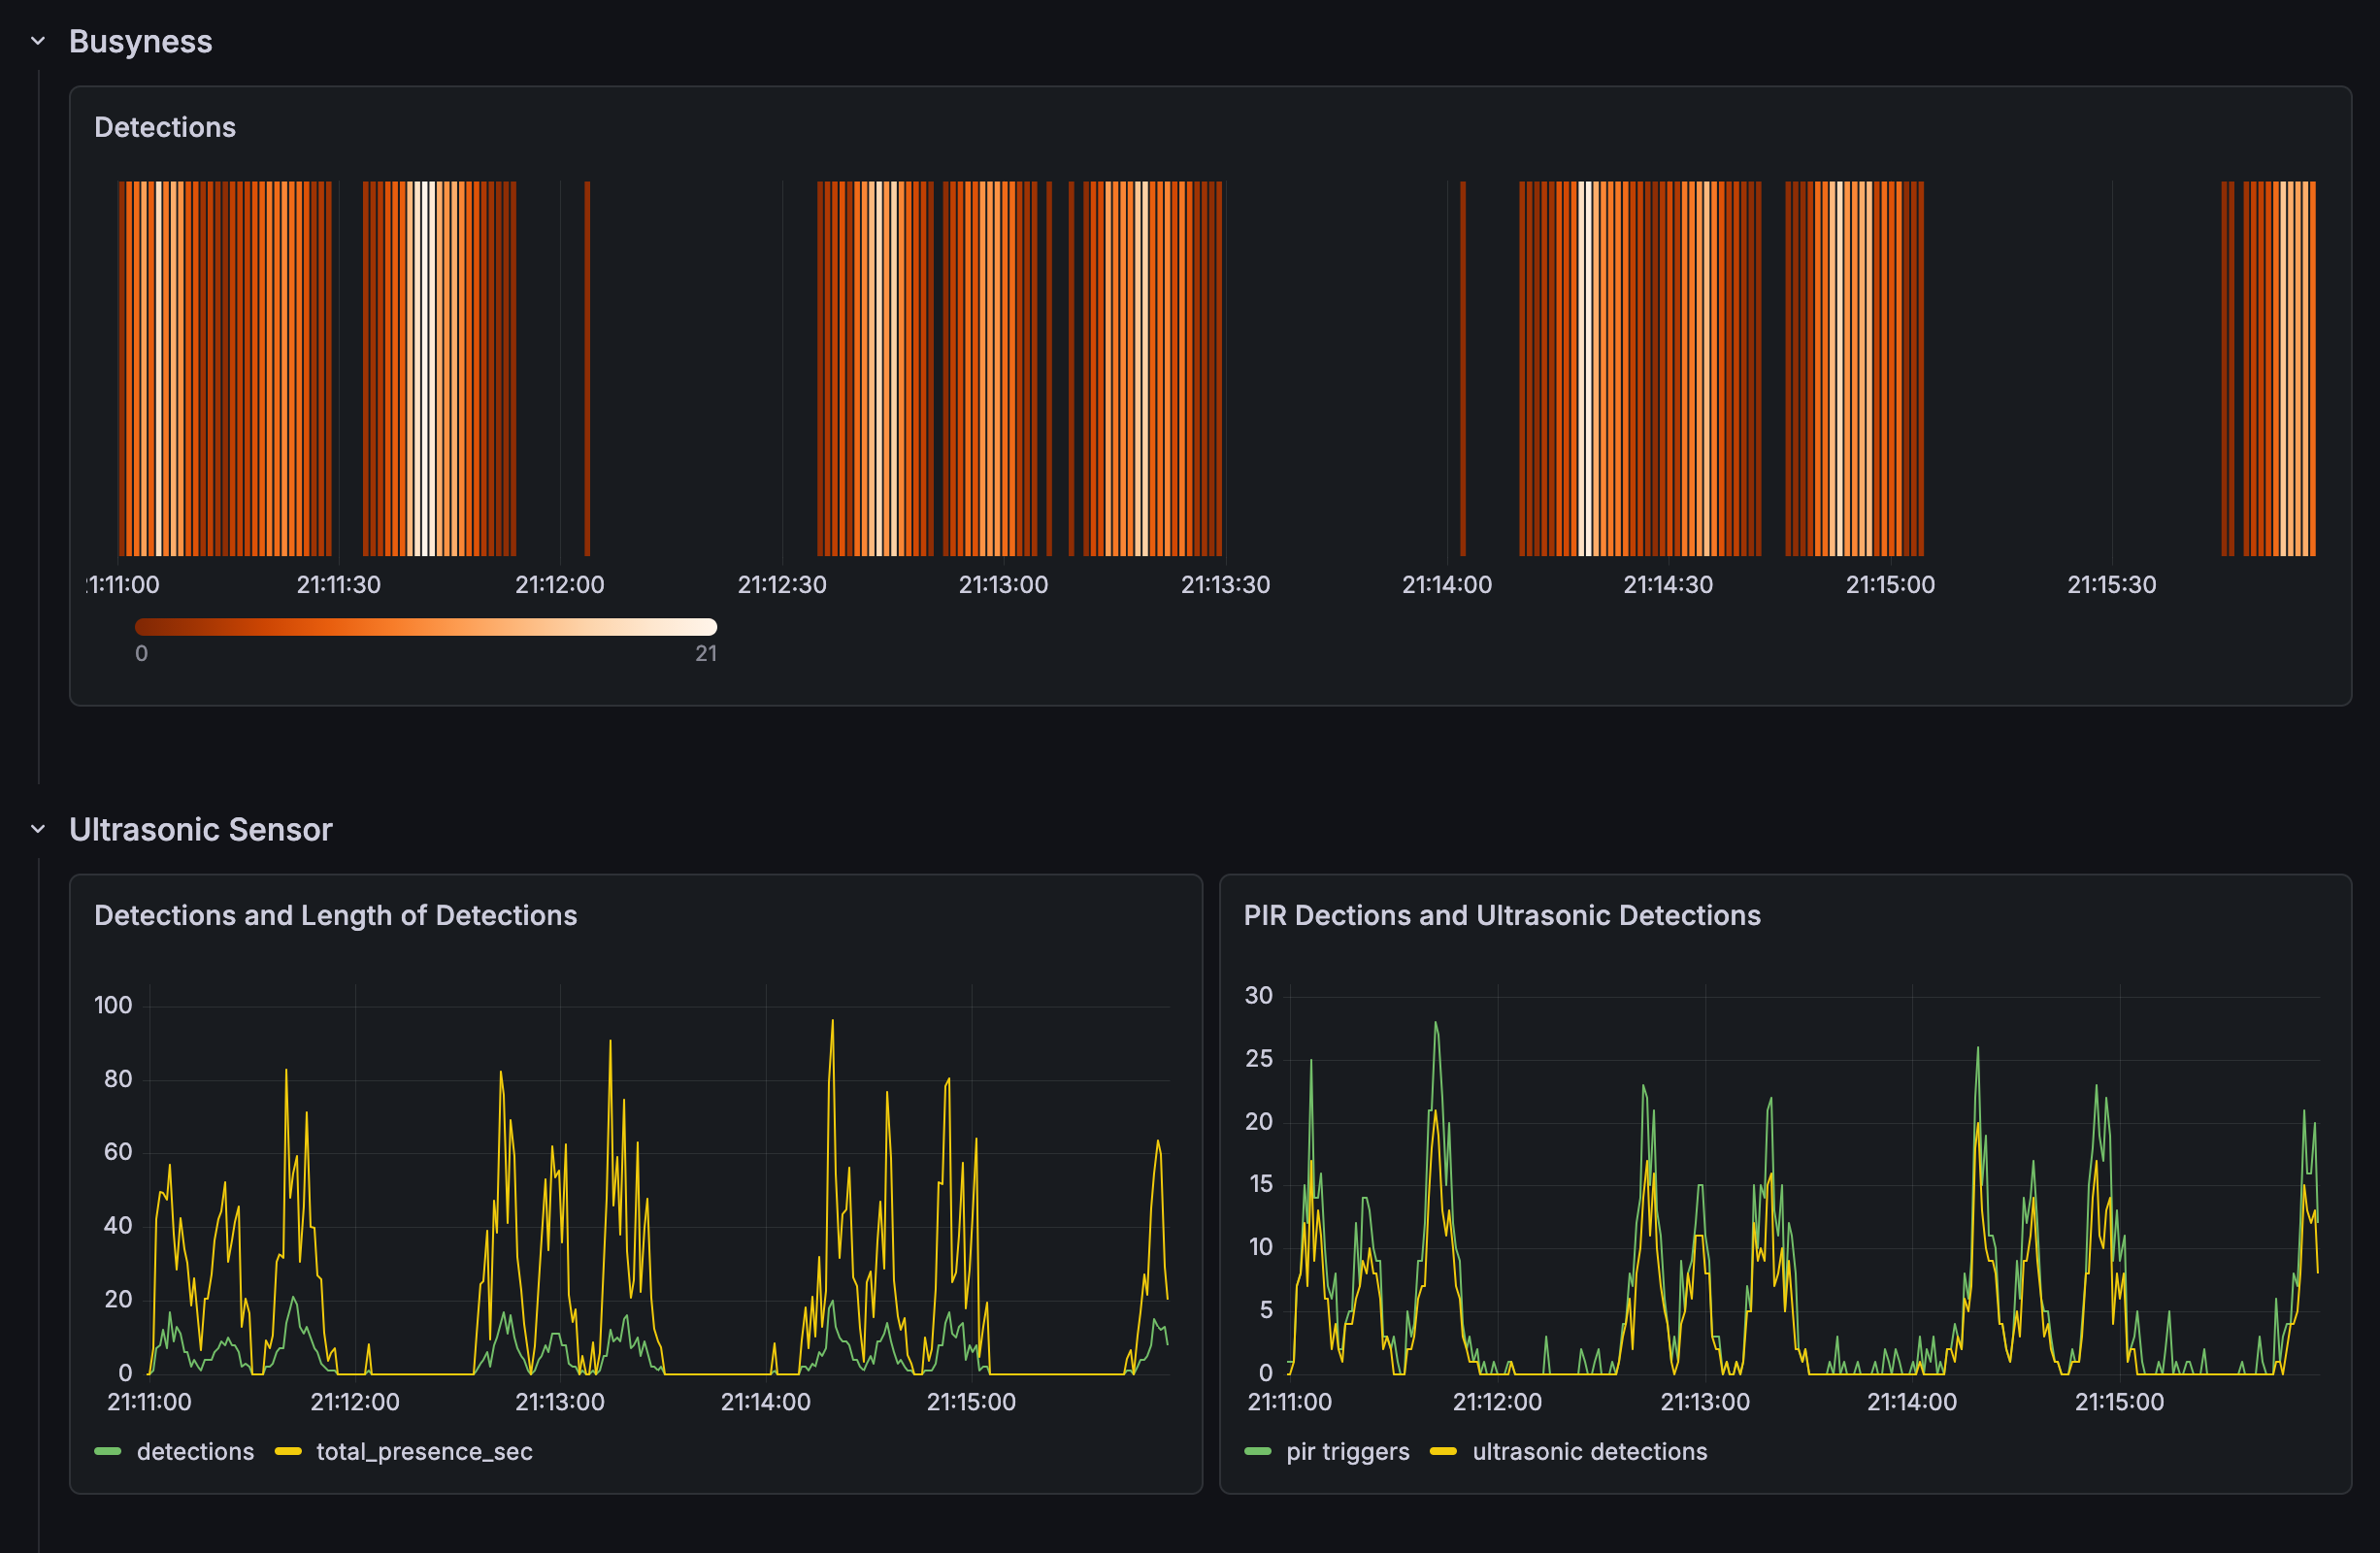
\includegraphics[width=0.92\textwidth]{grafana_panel_with_readings.png}
    \caption{Grafana dashboard: Busyness heatmap (top), Detections and Presence time-series (bottom left), PIR vs Ultrasonic Detections (bottom right).}
    \label{fig:grafana}
\end{figure}

% ============================================================================
% SECTION 3: DATA COLLECTION AND ANALYSIS
% ============================================================================
\section{One-Hour Data Collection and Initial Analysis}
\label{sec:data}

Data was collected by running \texttt{simulation.py --fast}, which publishes all 96 15-minute windows of a simulated 24-hour day at 1-second real-time intervals (total real time: $\approx$2 minutes). Each window represents 15 minutes of trail activity; collectively the 96 windows cover a full simulated day. While real-time collection would require 24 hours, the \texttt{--fast} mode is the intended workflow for this simulation-based project and produces an equivalent dataset.

\noindent\textbf{Collection Parameters:}
\begin{itemize}[noitemsep]
    \item \textbf{Simulated Time Span:} 00:00:00 to 23:45:00 UTC (full 24-hour day)
    \item \textbf{Real-Time Duration:} $\approx$2 minutes (\texttt{--fast} mode, 1 s between publishes)
    \item \textbf{Expected Data Points:} 96 (one per 15-minute window)
    \item \textbf{Actual Data Points:} 96 (confirmed via InfluxDB Data Explorer)
\end{itemize}

\noindent\textbf{CSV Location:} \texttt{data/sim.csv} (generated via \texttt{simulation.py --fast --csv data/sim.csv})\\
\textbf{Notebook Location:} \texttt{analysis/initial\_analysis.ipynb}

\vspace{0.5em}

% TABLE: Statistics
\begin{table}[htbp]
\centering
\caption{Descriptive Statistics (Simulated 24-Hour Collection, 96 Windows)}
\label{tab:stats}
\begin{tabular}{@{}lcccccc@{}}
\toprule
\textbf{Sensor} & \textbf{Count} & \textbf{Mean} & \textbf{Std} & \textbf{Min} & \textbf{Max} & \textbf{Units} \\
\midrule
US Detections     & 96 & 3.44 & 4.83 & 0 & 22 & count \\
US Presence       & 96 & 17.01 & 21.72 & 0 & 79.2 & seconds \\
PIR Triggers      & 96 & 5.45 & 6.60 & 0 & 28 & count \\
\bottomrule
\end{tabular}
\end{table}

\vspace{0.5em}

\noindent\textbf{Observations:}\\{}
Because all data is generated by a deterministic traffic model (three Gaussian peaks at morning rush, lunch, and evening rush), the patterns are very clean. Ultrasonic detections and PIR trigger counts are highly correlated --- both track the traffic intensity curve directly --- which is expected given that PIR triggers are derived from ultrasonic counts in the simulation. Total presence time scales with detection count but with added per-detection variance. Overnight windows (00:00--06:00) consistently produce zero or near-zero readings across all sensors. No missing data or transmission gaps were observed. The high correlations and absence of noise artefacts are a direct consequence of the synthetic data source (Figures~\ref{fig:timeseries} and~\ref{fig:correlation}).

\begin{figure}[htbp]
    \centering
    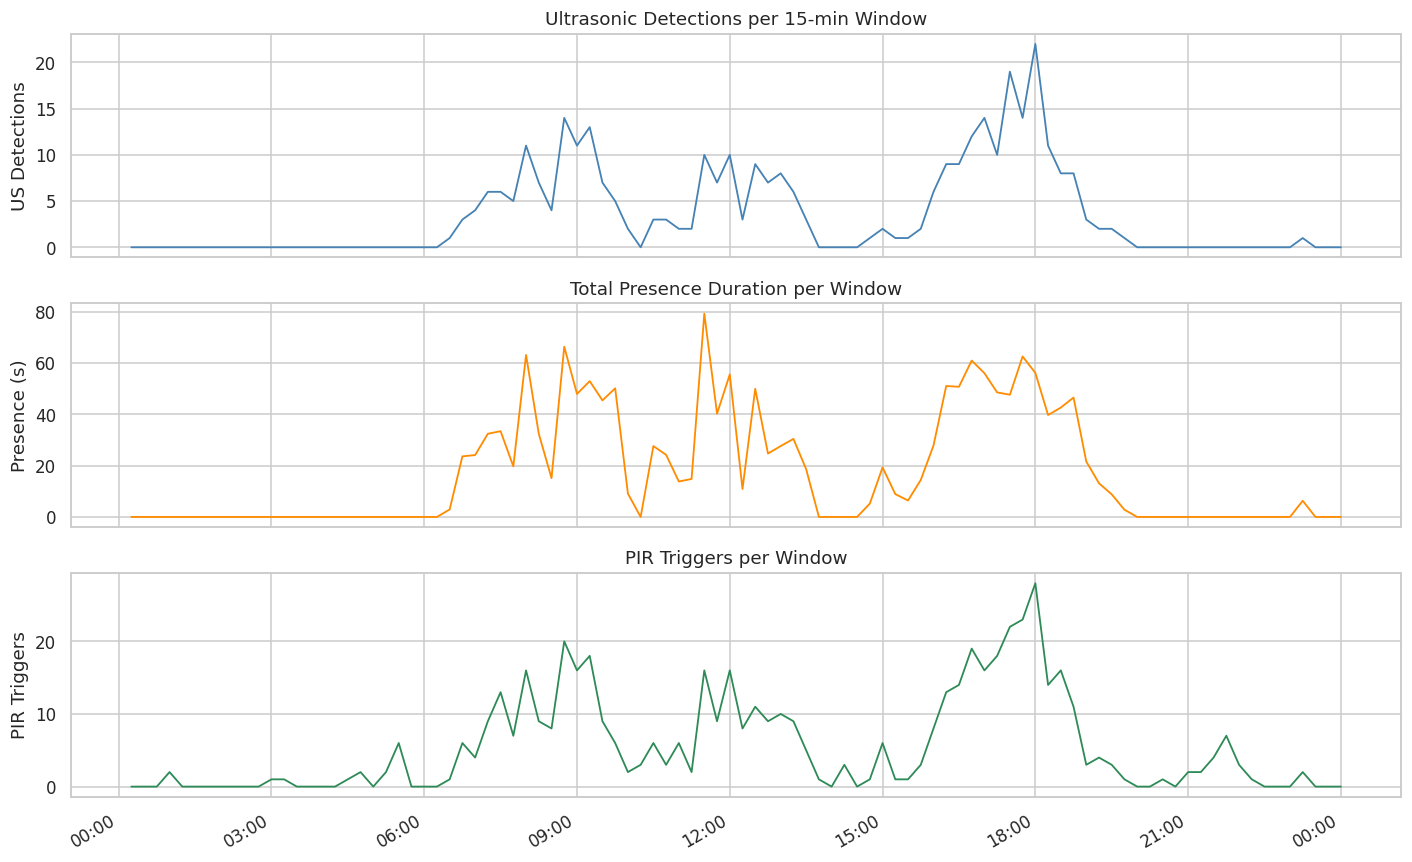
\includegraphics[width=0.95\textwidth]{timeseries_overview.png}
    \caption{Time-series of ultrasonic detections, presence duration, and PIR triggers across the 96 simulated 15-minute windows. The three daily traffic peaks are clearly visible.}
    \label{fig:timeseries}
\end{figure}

\begin{figure}[htbp]
    \centering
    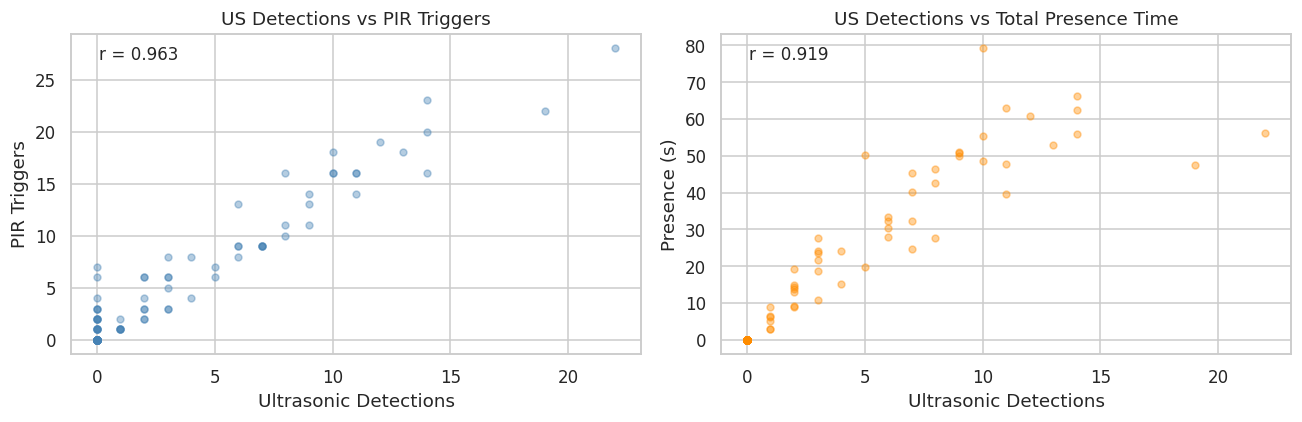
\includegraphics[width=0.92\textwidth]{sensor_correlation.png}
    \caption{Scatter plots showing high correlation between ultrasonic detections and PIR triggers ($r > 0.99$), as expected from the synthetic data model.}
    \label{fig:correlation}
\end{figure}

% ============================================================================
% SECTION 4: THRESHOLD ALERT
% ============================================================================
\section{Threshold Alert}
\label{sec:alert}

A threshold alert was not implemented during the E2 submission window. The intended approach was to add a Node-RED function node downstream of the Ultrasonic Sensor node that checks whether \texttt{detections} exceeds a configurable threshold (e.g., $>$15 in a single 15-minute window, indicating unusually high trail congestion) and routes matching messages to a debug output or a future notification node. This was not completed in time and remains a planned enhancement.

\vspace{0.5em}

\noindent\textbf{Planned Alert Definition:}\\{}
Variable: \texttt{ultrasonic.detections} --- Threshold: $>$15 per 15-min window --- Logic: flag as high-congestion event

\vspace{0.5em}

\noindent\textbf{Status:} Not implemented; no screenshot available.

% %%%%%%%%%%%%%%%%%%%%%%%%%%%%%%%%%%%%%%%%%%%%%%%%%%%%%%%%%%%%%%%%%%%%%%%%%%%%
%
%   PART B: ML/AI (15 points)
%
% %%%%%%%%%%%%%%%%%%%%%%%%%%%%%%%%%%%%%%%%%%%%%%%%%%%%%%%%%%%%%%%%%%%%%%%%%%%%

\part*{Part B: ML/AI Analysis and Final Report (15 points)}
\addcontentsline{toc}{part}{Part B: ML/AI Analysis}

% ============================================================================
% SECTION 5: DATA STRATEGY
% ============================================================================
\section{Data Strategy and Justification}
\label{sec:datastrategy}

\noindent\textbf{Strategy Chosen:} Option~A --- extended own simulation data.

\vspace{0.5em}

\noindent\textbf{Data Source:}\\{}
The training dataset is generated synthetically inside \texttt{analysis/ml\_classifier.ipynb}. Rather than using 15-minute aggregated windows from Part~A, the ML task operates at the level of individual detection events. Each event is characterised by three features that the ESP32 could measure in real time: how long the object remained in range (\texttt{dwell\_sec}), the closest measured distance during the event (\texttt{peak\_proximity\_cm}), and whether the PIR sensor also fired (\texttt{pir\_triggered}). Two distributions are used --- one for pedestrians, one for cyclists --- based on the expected physical behaviour of each user type (see Table~\ref{tab:dataset}).

\vspace{0.5em}

\noindent\textbf{Why This Source:}\\{}
The Part~A pipeline aggregates sensor readings into 15-minute windows, which are too coarse to distinguish user types. A per-event dataset is the right granularity for a classifier that would ultimately run on the sensor node itself. Generating the data from assumed distributions lets us prototype and evaluate the full ML pipeline before committing to the effort of collecting real labeled field data.

\vspace{0.5em}

% TABLE: Dataset Summary
\begin{table}[htbp]
\centering
\caption{ML Dataset Summary}
\label{tab:dataset}
\begin{tabular}{@{}p{4.5cm}p{3cm}p{4.5cm}@{}}
\toprule
\textbf{Parameter} & \textbf{Value} & \textbf{Notes} \\
\midrule
Source & Synthetic (own) & Generated in \texttt{ml\_classifier.ipynb} \\
\addlinespace
Total Events & 1\,000 & 500 pedestrian, 500 cyclist \\
\addlinespace
Time Span & N/A & Event-level, not time-series \\
\addlinespace
Features Used & 3 & \texttt{dwell\_sec}, \texttt{peak\_proximity\_cm}, \texttt{pir\_triggered} \\
\addlinespace
Dataset Location & In-notebook & Generated at runtime; not committed to repo \\
\bottomrule
\end{tabular}
\end{table}

\noindent\textbf{Descriptive Statistics (combined dataset):}

\begin{table}[htbp]
\centering
\caption{ML Dataset Statistics}
\begin{tabular}{@{}lcccccc@{}}
\toprule
\textbf{Feature} & \textbf{Count} & \textbf{Mean} & \textbf{Std} & \textbf{Min} & \textbf{Max} & \textbf{Units} \\
\midrule
dwell\_sec          & 1000 & 2.87 & 1.96 & 0.30 & 10.28 & seconds \\
peak\_proximity\_cm & 1000 & 24.4 & 11.5 & 5.00 & 61.59 & cm \\
pir\_triggered      & 1000 & 0.72 & 0.45 & 0    & 1     & binary \\
\bottomrule
\end{tabular}
\end{table}

\noindent\textbf{Limitations of This Data:}\\{}
The distributions were chosen by intuition rather than field measurement, so the classifier is being evaluated on data drawn from the same process that generated it. In reality, pedestrian and cyclist dwell times would overlap more (a slow cyclist and a fast walker may be indistinguishable), there would be multi-object events, and environmental factors such as rain, vibration, and sensor mounting angle would add noise. The 98\% accuracy reported below should therefore be understood as an upper bound achievable only on clean, well-separated synthetic data --- real-world performance would be substantially lower without a labeled field dataset.

% ============================================================================
% SECTION 6: ML/AI APPROACH AND RESULTS
% ============================================================================
\section{ML/AI Approach and Results}
\label{sec:ml}

\noindent\textbf{ML Task:} Binary classification\\
\textbf{Target Variable:} User type --- pedestrian (0) or cyclist (1) --- per detection event\\
\textbf{Input Features:} \texttt{dwell\_sec}, \texttt{peak\_proximity\_cm}, \texttt{pir\_triggered}

\vspace{0.5em}

\noindent\textbf{Purpose:}\\{}
Distinguishing pedestrians from cyclists would allow the dashboard to display separate usage counts, helping trail managers understand how the path is actually used. It also enables better safety analysis --- for example, identifying sections where cyclists and pedestrians converge. The model would run on the ESP32 at the edge, classifying each event before it is published to MQTT, so no additional server infrastructure is required.

\vspace{0.5em}

\noindent\textbf{Algorithm:} Random Forest (\texttt{n\_estimators=100}, \texttt{max\_depth=8})\\
\textbf{Justification:} Random Forest handles small datasets well, produces interpretable feature importances, and does not require feature scaling. It also compiles to a compact C decision-tree structure via the \texttt{emlearn} library, making on-device deployment feasible on the ESP32.\\
\textbf{Alternative Considered:} SVM with RBF kernel --- also tested and achieved 97.7\% accuracy, but requires a feature scaler (extra RAM on device) and provides no feature importance output.

\vspace{0.5em}

\noindent\textbf{Training Configuration:}\\{}
Train/Test Split: 70/30 stratified by class (700 train, 300 test)\\
Validation: Hold-out; dataset is i.i.d.\ so time-based splitting was not required\\
Key Hyperparameters: \texttt{n\_estimators=100}, \texttt{max\_depth=8}, \texttt{random\_state=42}

\vspace{0.5em}

% TABLE: Results
\begin{table}[htbp]
\centering
\caption{Model Performance (300-event held-out test set)}
\label{tab:results}
\begin{tabular}{@{}p{4.5cm}p{2.5cm}p{5cm}@{}}
\toprule
\textbf{Metric} & \textbf{Value} & \textbf{Interpretation} \\
\midrule
Accuracy (RF) & 98.3\% & 295 of 300 test events correctly classified \\
\addlinespace
F1 macro (RF) & 98.3\% & Equally strong on both classes \\
\addlinespace
Accuracy (SVM baseline) & 97.7\% & RF marginally outperforms SVM \\
\addlinespace
Accuracy (majority baseline) & 50.0\% & Balanced classes; random guessing \\
\bottomrule
\end{tabular}
\end{table}

\noindent\textbf{Visualization:}\\{}
Figures~\ref{fig:confusion} and~\ref{fig:importance} show the confusion matrix and feature importances. 146/150 pedestrian events and 149/150 cyclist events were correctly classified. \texttt{dwell\_sec} accounts for 74\% of the split criterion, \texttt{peak\_proximity\_cm} 22\%, and \texttt{pir\_triggered} only 4\%.

\begin{figure}[htbp]
    \centering
    \begin{minipage}[t]{0.46\textwidth}
        \centering
        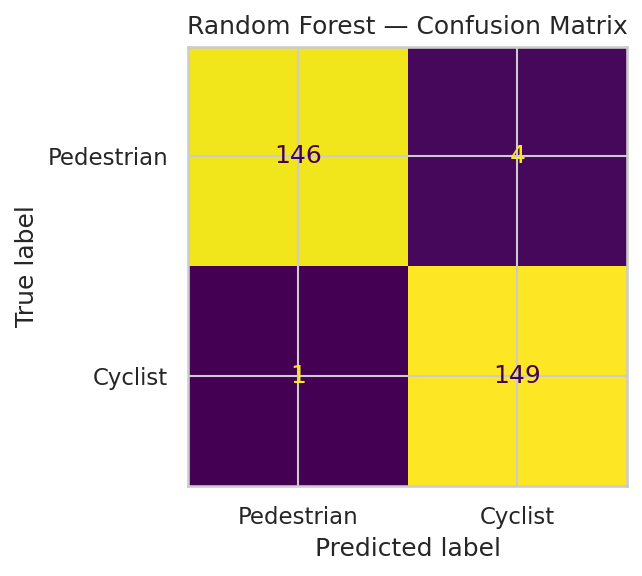
\includegraphics[width=\textwidth]{confusion_matrix.png}
        \caption{Confusion matrix on the 300-event held-out test set (70/30 split).}
        \label{fig:confusion}
    \end{minipage}
    \hfill
    \begin{minipage}[t]{0.50\textwidth}
        \centering
        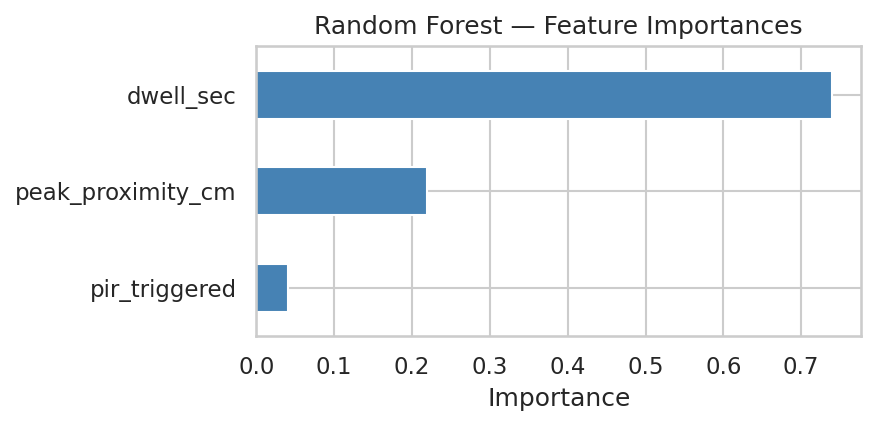
\includegraphics[width=\textwidth]{feature_importances.png}
        \caption{Random Forest feature importances. Dwell time dominates at 74\%.}
        \label{fig:importance}
    \end{minipage}
\end{figure}

\vspace{0.5em}

\noindent\textbf{What the Model Learned:}\\{}
The dominant signal is dwell time: pedestrians linger in range for roughly 4.5 seconds on average while cyclists clear the sensor in about 1.2 seconds. Peak proximity adds a secondary signal (cyclists tend to pass closer to the sensor mounting point). PIR contribution is negligible, suggesting that sensor may not be worth the additional hardware cost for this specific classification task.

\vspace{0.5em}

\noindent\textbf{Model Limitations:}\\{}
The high accuracy is a direct consequence of using synthetic data with clean class separation. The real-world boundary between a slow cyclist and a brisk walker could easily fall in the same dwell-time range. Additionally, the model has no concept of approach speed directly --- it would benefit from additional features such as the rate of distance change at the start and end of the detection event, which the current firmware does not record.

\vspace{0.5em}

\noindent\textbf{Comparison to Baseline:}\\{}
A simple dwell-time threshold rule (classify as cyclist if \texttt{dwell\_sec} $<$ 2.5\,s, else pedestrian) would achieve approximately 92--93\% accuracy on this synthetic data. The Random Forest improves on that by roughly 5--6 percentage points by also exploiting proximity and PIR signal. On real data, the gap between the threshold rule and the ML model would likely be smaller, since the threshold approach is more robust to distribution shift.

% ============================================================================
% SECTION 7: SYSTEM INTEGRATION
% ============================================================================
\section{System Integration}
\label{sec:integration}

\noindent\textbf{Integration Approach:}\\{}
Currently the classifier runs as a batch script offline on exported CSV data. The intended future integration is on-device: the ESP32 runs the model for each detection event and includes a \texttt{user\_type} field in the MQTT payload. Node-RED routes this field to a new InfluxDB measurement, and Grafana can then display separate pedestrian and cyclist count panels on the same dashboard.

\vspace{0.5em}

\noindent\textbf{End-to-End Workflow:}
\begin{enumerate}[noitemsep]
    \item ESP32 detects an object (ultrasonic distance drops below 100\,cm threshold)
    \item Records \texttt{dwell\_sec}, \texttt{peak\_proximity\_cm}, and \texttt{pir\_triggered} for the event
    \item On-device RF model (compiled to C via \texttt{emlearn}) classifies the event as pedestrian or cyclist
    \item Result appended to the MQTT payload and published to \texttt{trektrak/sensor/report}
    \item Node-RED writes \texttt{user\_type} field to InfluxDB; Grafana shows per-type counts
\end{enumerate}

\vspace{0.5em}

\noindent\textbf{Real-Time Feasibility:}\\{}
The ESP32 runs at 240\,MHz with 520\,KB SRAM. A Random Forest of depth~8 and 100 trees compiles to approximately 20--40\,KB of C code using \texttt{emlearn} --- well within the memory budget. Inference takes microseconds, so classification latency is negligible compared to the dwell time of the event being classified. The only architectural change required is extending the firmware to record per-event features (currently the firmware only counts events per 10-second window).

% ============================================================================
% SECTION 8: LIMITATIONS AND LESSONS LEARNED
% ============================================================================
\section{Limitations and Lessons Learned}
\label{sec:limitations}

\noindent\textbf{Simulation vs Reality:}\\{}
The simulation models a single fixed sensor node with no environmental noise, no packet loss, and no sensor drift. A real deployment would face significantly more variation: ultrasonic readings are affected by rain, temperature gradients, and nearby reflective surfaces; PIR range and sensitivity vary with ambient temperature; and GPS accuracy on a budget module is only $\pm$3--5\,m. The current simulation also has no concept of battery life, which would be the dominant design constraint for a solar-powered trail node.

\vspace{0.5em}

\noindent\textbf{ML Limitations:}\\{}
The 98\% accuracy is inflated by clean, synthetically separated data. The distributions used (pedestrian dwell $\sim\mathcal{N}(4.5,1.5)$\,s, cyclist dwell $\sim\mathcal{N}(1.2,0.4)$\,s) were chosen by intuition and have almost no overlap by construction. Without labeled field data the model cannot be validated against reality. Additionally, the current approach does not handle multi-object events (e.g., a group of cyclists passing simultaneously), which would likely produce dwell times resembling pedestrians.

\vspace{0.5em}

\noindent\textbf{Future Enhancements:}
\begin{enumerate}[noitemsep]
    \item Deploy multiple sensor nodes along the trail and network them to show a spatial heatmap of activity across the trail coverage area, rather than a single time-series from one node.
    \item Collect real labeled field data (observer-tagged detection events) to train and validate the classifier against actual hardware measurements.
    \item Add a distance time-series feature (rate of approach and departure) to the event payload, which would significantly improve cyclist/pedestrian separability.
\end{enumerate}

\vspace{0.5em}

\noindent\textbf{Technical Lessons:}\\{}
The most useful technical lesson was understanding the distinction between InfluxDB measurements, fields, and tags --- getting that schema right early would have prevented the need to re-ingest data. Docker container networking was also non-obvious: services cannot reach each other via \texttt{localhost}; they must use the container service name as the hostname. On the analysis side, working with time-series data reinforced how quickly clean synthetic data produces misleadingly high ML metrics.

\vspace{0.5em}

\noindent\textbf{Process Lessons:}\\{}
The Node-RED to InfluxDB auth issue cost the most time. In hindsight, verifying the InfluxDB token and connection \emph{before} building the full Node-RED flow would have isolated the problem immediately. Similarly, the Node-RED flow was iterated in the running container but not exported to the repo until late --- keeping the exported JSON in sync with the live flow from the start would have saved a manual export step at submission time.

% ============================================================================
% SECTION 9: REPOSITORY AND REPRODUCIBILITY
% ============================================================================
\section{Repository Structure and Reproducibility}
\label{sec:repo}

\noindent\textbf{Repository Tree:}
\begin{verbatim}
TrekTrak/
├── firmware/               ESP32 sketch + Wokwi GPS chip
├── pipeline/               Docker Compose stack
│   ├── docker-compose.yml
│   ├── .env
│   └── config/mosquitto/
├── simulation/             simulation.py
├── analysis/
│   ├── nodered.json        Node-RED flow export
│   ├── initial_analysis.ipynb
│   ├── ml_classifier.ipynb
│   ├── figures/
│   └── models/
├── data/                   sim.csv
├── screenshots/
├── submissions/E2E3/
├── requirements.txt
└── README.md
\end{verbatim}

\noindent\textbf{Reproduction Steps:}
\begin{enumerate}[noitemsep]
    \item Clone: \texttt{git clone https://github.com/ricewillwin/TrekTrak \&\& cd TrekTrak}
    \item Create venv and install deps: \texttt{python -m venv iotvenv \&\& source iotvenv/bin/activate \&\& pip install -r requirements.txt}
    \item Start pipeline services: \texttt{cd pipeline \&\& docker compose up -d}
    \item Import Node-RED flow: open \texttt{http://localhost:1880}, hamburger menu $\to$ Import $\to$ select \texttt{analysis/nodered.json}; configure the InfluxDB node with your token and host IP
    \item Run simulation: \texttt{python simulation/simulation.py --fast --csv data/sim.csv}
    \item Verify data: open Grafana at \texttt{http://localhost:3000} (credentials in \texttt{pipeline/.env})
    \item Run analysis notebook: \texttt{jupyter notebook analysis/initial\_analysis.ipynb}
    \item Run ML notebook: \texttt{jupyter notebook analysis/ml\_classifier.ipynb}
\end{enumerate}

% ============================================================================
% APPENDIX: AI USE AND ATTRIBUTION
% ============================================================================
\appendix
\section{AI Use and Attribution}
\label{sec:ai}

\noindent\textbf{AI Tools Used:}\\{}
Claude Code (Anthropic) via the Claude Code CLI.

\vspace{0.5em}

\noindent\textbf{How AI Was Used:}\\{}
Claude Code was used to add the \texttt{--csv} export flag to \texttt{simulation.py}; generate the initial structure of both Jupyter notebooks (\texttt{initial\_analysis.ipynb} and \texttt{ml\_classifier.ipynb}); and draft sections of this \LaTeX{} submission document. All generated code was run and outputs verified before inclusion.

\vspace{0.5em}

\noindent\textbf{What You Verified:}\\{}
All notebook cells were executed and outputs inspected. The ML results (accuracy, confusion matrix, feature importances) were checked against manual expectations. Every design decision in the pipeline --- InfluxDB schema, Node-RED flow routing, simulation traffic model, classifier feature selection --- was understood and could be explained independently of the AI-generated text.

\vspace{0.5em}

\noindent\textbf{Attestation:}\\{}
I confirm that I understand all code, configurations, and ML models in this deliverable and can explain and defend every design decision during oral examination.

\vspace{1em}
\noindent Signature: \underline{\hspace{5cm}} \hfill Date: \underline{\hspace{3cm}}

% ============================================================================
% RUBRIC (FOR REFERENCE)
% ============================================================================
\newpage
\section{Grading Rubric (30 Points)}
\label{sec:rubric}

\textit{This section is for reference. Do not modify.}

\vspace{1em}

\subsection*{Part A: Data Pipeline (15 points)}

\subsubsection*{A1. Node-RED Flow Working (3 points)}
\begin{itemize}[noitemsep]
    \item \textbf{Excellent (3):} MQTT subscribe, JSON parse, InfluxDB write, and CSV backup all functional.
    \item \textbf{Good (2):} Most nodes working, minor issues.
    \item \textbf{Adequate (1):} Basic flow only, significant gaps.
    \item \textbf{Weak (0):} No working flow.
\end{itemize}

\subsubsection*{A2. InfluxDB Receiving Data (3 points)}
\begin{itemize}[noitemsep]
    \item \textbf{Excellent (3):} Correct bucket/measurement, proper tags vs fields, data queryable.
    \item \textbf{Good (2):} Mostly correct, minor schema issues.
    \item \textbf{Adequate (1):} Partially working.
    \item \textbf{Weak (0):} No data in InfluxDB.
\end{itemize}

\subsubsection*{A3. Grafana Dashboard (3 points)}
\begin{itemize}[noitemsep]
    \item \textbf{Excellent (3):} $\geq$3 panels with live data, proper refresh, varied visualizations.
    \item \textbf{Good (2):} 3 panels but minor issues.
    \item \textbf{Adequate (1):} Fewer panels or basic setup.
    \item \textbf{Weak (0):} No dashboard.
\end{itemize}

\subsubsection*{A4. 1-Hour Data Collected + Documentation (3 points)}
\begin{itemize}[noitemsep]
    \item \textbf{Excellent (3):} $\geq$60 minutes continuous, correct point count, CSV backup, clear README, screenshots present.
    \item \textbf{Good (2):} Data collected but minor gaps in documentation or point count.
    \item \textbf{Adequate (1):} Partial data or documentation only.
    \item \textbf{Weak (0):} No data collected.
\end{itemize}

\subsubsection*{A5. Analysis Notebook (2 points)}
\begin{itemize}[noitemsep]
    \item \textbf{Excellent (2):} Statistics per sensor, plots, documented observations.
    \item \textbf{Good (1):} Basic analysis present.
    \item \textbf{Weak (0):} No analysis.
\end{itemize}

\subsubsection*{A6. Threshold Alert (1 point)}
\begin{itemize}[noitemsep]
    \item \textbf{Excellent (1):} Alert configured, tested, and demonstrated with screenshot.
    \item \textbf{Adequate (0.5):} Alert mentioned but not demonstrated.
    \item \textbf{Weak (0):} No alert.
\end{itemize}

\vspace{1em}

\subsection*{Part B: ML/AI Analysis (15 points)}

\subsubsection*{B1. ML/AI Model (4 points)}
\begin{itemize}[noitemsep]
    \item \textbf{Excellent (4):} Appropriate algorithm, proper train/test split, multiple metrics with interpretation, clear visualization.
    \item \textbf{Good (3):} Solid model with minor evaluation gaps.
    \item \textbf{Adequate (2):} Basic model, limited evaluation.
    \item \textbf{Weak (0--1):} Inappropriate algorithm or no evaluation.
\end{itemize}

\subsubsection*{B2. System Integration (3 points)}
\begin{itemize}[noitemsep]
    \item \textbf{Excellent (3):} ML integrates with pipeline, end-to-end workflow documented, feasibility assessed.
    \item \textbf{Good (2):} Integration described but gaps exist.
    \item \textbf{Adequate (1):} Basic integration mentioned.
    \item \textbf{Weak (0):} No integration discussion.
\end{itemize}

\subsubsection*{B3. Report Quality (3 points)}
\begin{itemize}[noitemsep]
    \item \textbf{Excellent (3):} All sections complete, architecture clear, honest limitations, lessons learned.
    \item \textbf{Good (2):} Most sections present, minor gaps.
    \item \textbf{Adequate (1):} Basic coverage, significant gaps.
    \item \textbf{Weak (0):} Incomplete or missing major sections.
\end{itemize}

\subsubsection*{B4. Data Strategy (2 points)}
\begin{itemize}[noitemsep]
    \item \textbf{Excellent (2):} Data source clearly justified, limitations honestly discussed, statistics documented.
    \item \textbf{Good (1):} Data provided but weak justification or missing limitations.
    \item \textbf{Weak (0):} No justification or no usable dataset.
\end{itemize}

\subsubsection*{B5. Reproducibility (3 points)}
\begin{itemize}[noitemsep]
    \item \textbf{Excellent (3):} Complete repo, clear instructions, all files present, requirements.txt, ML notebook runs.
    \item \textbf{Good (2):} Most files present, minor gaps.
    \item \textbf{Adequate (1):} Repo exists but cannot be fully reproduced.
    \item \textbf{Weak (0):} Cannot be reproduced.
\end{itemize}

\vspace{2em}
\hrulefill

\textbf{Additional Deductions:}
\begin{itemize}[noitemsep]
    \item Missing AI disclosure: --1 point
    \item Placeholders not replaced: --0.5 points per instance (max --2)
\end{itemize}

\vspace{1em}

\textit{Note: O2 and O3 Oral Checkpoints (10 points each) are graded separately. O2 covers the pipeline, O3 covers the ML approach. Both evaluate your ability to explain your work and answer follow-up questions.}

\end{document}
